\documentclass[a4paper,10pt]{article}
\usepackage[top=2.5cm,bottom=2.5cm,left=2.5cm,right=2.5cm,showframe]{geometry}
\usepackage{xcolor,fancyhdr}
\usepackage{tikz}
\usepackage{amsmath,amssymb,amsthm,amsfonts}
\usepackage{stmaryrd}

\usepackage{lineno}
\linenumbers
\setpagewiselinenumbers

%%%%%%%%%%%%%  PLEASE DO NOT EDIT ANY OF THE LINES ABOVE %%%%%%%%%%%%%%%
% Insert your text between "\begin{document}" and "\end{document}" below. 
% The total length of your summary notes should not exceed 2 sides of a
% single sheet of A4, with maximum 58 lines of text per page.
%%%%%%%%%%%%%%%%%%%%%%%%%%%%%%%%%%%%%%%%%%%%%%%%%%%%%%%%%%%%%%%%%%%%%%%%

\usepackage{mathtools}
\usepackage{graphicx}
\graphicspath{ {./} }
\usepackage{wrapfig}
\newcommand{\Parsep}{\rule{6cm}{0.4pt}}
\newcommand{\tab}{\hspace{0.5cm}}
\newcommand{\uv}{\mathbf{u}}
\newcommand{\gv}{\mathbf{g}}
\newcommand{\zv}{\mathbf{0}}
\newcommand{\wv}{\mathbf{w}}
\newcommand{\nv}{\mathbf{n}}
\newcommand{\const}{\text{const.}}

\begin{document}

\include{stylefile}


Euler Equations:
\tab\tab\tab
$\frac{D}{Dt} = \frac{\partial}{\partial t} + (\uv \cdot \nabla)$ \tab
RTT: $\frac{d}{dt}\iiint_{V(t)} f dV = \iiint_{V(t)} \frac{\partial f}{\partial t} + \nabla \cdot (f \uv) dV$

(i) $\frac{\partial \rho}{\partial t} + \nabla \cdot (\rho \uv) = 0$ 
(ii) $\rho \frac{D \uv}{D t} = -\nabla p + \rho \gv$ 
(iii) $\rho c_v \frac{D T}{D t} = -p \nabla \cdot \uv + p q$ 
(iv) $p=\rho R T$, $pV=MRT$

(v) $\gamma \coloneqq \frac{c_p}{c_v} = 1+\frac{R}{c_v}$,
$\rho q = \frac{p}{\gamma -1} \frac{D}{Dt}\left( \log \left( \frac{p}{\rho^\gamma} \right) \right)$,
$q = T \frac{DS}{DT}$ ($S = S_0 + c_v \log \left( \frac{p}{\rho^\gamma} \right)$)

\underline{Incompressible}: $\frac{D\rho}{Dt} = 0 \Longrightarrow \nabla \cdot \uv = 0$ \tab
\underline{Irrotational}: $\nabla \wedge \uv = 0 \Longrightarrow \uv = \nabla \phi$ where $\nabla^2 \phi = 0$

\underline{Bernoulli}: $\phi_t + \frac{1}{2} {|\nabla \phi|}^{2} + \frac{p}{\rho} + \chi = F(t)$ (Often $\chi = gz = g\eta$)

\Parsep

\underline{Linear Wave Propagation} From $\rho = \rho_0 + \rho'$, $\uv = \zv + \uv'$, $p=p_0 + p'$

$\Longrightarrow p' = c_0^2 \rho'$ ($c_0^2 \coloneqq \frac{dp}{d\rho}(\rho_0)$), 

(ii) $\Longrightarrow \rho_0 {\uv'}_t = -\nabla p' = -c_0^2 \nabla \rho'$ ($\Longrightarrow \frac{\partial}{\partial t}(\nabla \wedge \wv) = \zv$)

(i) $\Longrightarrow {\rho '}_t + \rho_0 \nabla^2 \phi = 0$ (With prev, it implies $\phi_{tt} = c_0^2 \nabla^2 \phi$)

For $p'(0,t) = Ae^{-i \omega t}$, $p'(x,t) = f(x) e^{-i \omega t}$

\textbf{Conditions}: Radiation condition, Boundedness

\Parsep

\underline{Laplacian}:
2D: $\nabla^2 f(r) = \frac{1}{r} \frac{\partial}{\partial r}\left( r \frac{\partial f}{\partial r} \right)$ \tab
3D: $\nabla^2 f(r) = \frac{1}{r^2} \frac{\partial}{\partial r}\left( r^2 \frac{\partial f}{\partial r} \right)$

\underline{Mach}: $M \coloneqq \frac{U}{c_0}$ (Seek steady state (no dep on $t$)) $\phi_{xx} + \phi_{yy} = \stackrel{ \text{elim} p' \text{, expr in } \rho'}{\cdots}
\Longrightarrow (1-M^2) \phi_{xx}+\phi_{yy} = 0$
($U \mathbf{e}_x$ background flow)

\underline{Stokes Wave}
$\nabla^2 \phi = 0$

KBC: $\frac{D}{Dt} \left( z-\eta \right) = 0 \Longrightarrow \phi_z = \eta_t + \phi_x \eta_x + \phi_y \eta_y \stackrel{\text{Lin.}}{\Longrightarrow} \phi_z = \eta_t$ at $z=0$

DBC: Bernoulli $\Longrightarrow \phi_t + \frac{1}{2} {|\nabla \phi|}^2 + g \eta = 0 \stackrel{\text{Lin.}}{\Longrightarrow} \phi_t + g\eta = 0$ at $z=0$

No Flux: $\uv \cdot \nv = \mathbf{v}_B \cdot \nv$

Seek $\phi(x,z,t) = f(z) e^{i\left( kx - \omega t \right)}$, nontrivial solution.

\underline{Flowing fluid}: (BC) $\phi_z = \eta_t + U \eta_x$, $\phi_t + U \phi_x + g\eta = 0$ at $z=0$

\underline{Two fluids}: KBC: $\eta_t = \frac{\partial \phi_1}{\partial z} = \frac{\partial \phi_2}{\partial z}$ at $z=0$,
DBC: $\rho_1 \left( \frac{\partial \phi_1}{\partial t} + g\eta \right) = \rho_2 \left( \frac{\partial \phi_2}{\partial t} + g\eta \right)$ at $z=0$

\underline{Surface tension}: DBC: $\rho_1 (\frac{\partial \phi_1}{\partial t} + g\eta) - \rho_2 (\frac{\partial \phi_2}{\partial t} + g\eta) = \gamma \frac{\partial^2 \eta}{ {\partial x}^2}$ at $z=0$

\Parsep

\textbf{Internal Gravity, Strat. fluid} $\frac{D\rho}{Dt} = 0 \iff \nabla \cdot \uv = 0$ \tab
Seek perturb: $\uv = \zv$, $\rho = \rho_(z)$, $p=p_0 (z) \Longrightarrow p_0(z) = p_a - g\int_0^z \rho_0(\zeta) d\zeta$ (From momentum equ.)

Linearize: (i) $\rho'_t + w' \rho_0'(z) = 0$ \tab
(ii) $u'_x + v'_y + w'_z=0$ \tab
(iii) $\rho_0 u'_t = -p'_x$ \tab
(iv) $\rho_0 v'_t = -p'_y$ \tab
(v) $\rho_0 w'_t = -p'_z - \rho' g$

$\stackrel{\text{(iii),(iv)} \rightarrow \text{(ii)}}{\Longrightarrow} -p'_{xx} -p'_{yy} = \rho_0 {(u'_x+v'_y)}_t = -\rho_0 w'_{zt}$, \tab
$\stackrel{\text{(i)}\Longrightarrow\text{(v)}}{\Longrightarrow} \rho_0 w'_{tt} = -p'_{zt}-gp'_t = -p'_{zt} + gw' \rho_0'(z)$

$\stackrel{\text{Elim } p'}{\Longrightarrow} {(w'_{xx}+w'_{yy}+w'_{zz})}_{tt}=\frac{g}{\rho_0} \rho_0'(z) (w'_{xx}+w'_{yy}-\frac{1}{g}w'_{ztt})$

\Parsep

\textbf{Theory for Linear Waves}
$\phi_{tt} = c_0^2 \nabla^2 \phi$

$\frac{d^2 f}{{dr}^2} + \frac{1}{r} \frac{df}{dr} + (\frac{\omega}{c_0})^2 f = 0
\stackrel{\xi = kr, k=\frac{\omega}{c_0}}{\Longrightarrow}
\xi^2 \frac{d^2 f}{{d \xi}^2} + \xi \frac{df}{d\xi} + \xi^2 f = 0
\stackrel{|f| < \infty}{\Longrightarrow} f = A J_0 (\xi)
$

Take $\phi(x,y,z,t) = f(x)g(y)h(z) e^{-i \omega t}$

\textbf{Fourier Transform} $\hat f(k) = \int_{-\infty}^\infty f(x)e^{-ikx} dx$

IFT: $f(x) = \frac{1}{2\pi} \int_{-\infty}^\infty \hat f(k) e^{ikx} dk$, \tab
$\hat f(k) = \hat g (k) \hat h (k) \Longrightarrow f(x) = (g*h)(x) = \int_{-\infty}^\infty g(\xi)h(x-\xi) d\xi$

$\hat{\frac{d^n f}{{dx}^n}} = (ik)^n \hat f$

\Parsep

\textbf{Method of Stationary Phase} $\eta (Vt,t)$, eval asymptotically, then $V = \frac{x}{t}$.

$I(t) = \int_a^b f(k) e^{i \psi (k) t} dt$: $\psi'(k)$ simple zero at $k_*$, then
$I(t) \sim f(k_*) e^{i(\psi(k_*)t \pm \frac{\pi}{4})} \sqrt{\frac{2\pi}{|\psi''(k_*)|t}}$

Derivation: $I(t) = \int_a^{k_* - \epsilon} f(k) e^{i \psi (k)t} dk + \int_{k_* + \epsilon}^b f(k) e^{i\psi(k)t}dk + \int_{k_* - \epsilon}^{k_* + \epsilon} f(k) e^{i\psi(k)t}dk$

First and second terms $\sim O(\frac{1}{t})$ by Riemann-Lebesgue. By approxing $f(k) \sim f(k_*)$, $\psi(k) \sim \psi(k_*) + \frac{\psi''(k_*)}{2}(k-k_*)^2$,
$I(t) \sim \int_{k_*-\epsilon}^{k_*+\epsilon} f(k_*) e^{i\psi(k_*)t} \exp{(\frac{it\psi''(k_*)}{2}(k-k_*)^2)} dk + O(\frac{1}{t})$. With $k=k_* + s \sqrt{\frac{2}{t\psi''(k_*)}}$ for
$\psi''(k_*) > 0$, $I(t) \sim f(k_*) e^{i\psi(k_*)t} \sqrt{\frac{2}{\psi''(k_*)t}} \int_{-\epsilon \sqrt{\psi''(k_*)/2}}^{\epsilon \sqrt{\psi''(k_*)/2}} e^{is^2} ds + O(\frac{1}{t})$.
Contour integral, $I(t) \stackrel{t \rightarrow \infty}{\sim} (1+i)f(k_*) e^{i\psi(k_*)t} \sqrt{\frac{\pi}{\psi''(k_*)t}} + O(\frac{1}{t})$. Similarly with $\psi''(k_*) < 0$.
General result can be written.

For $\psi(k) = kV \mp \omega t$, \underline{Group velocity}: $c_g(k) \coloneqq \frac{d\omega}{dk}$ \tab
\underline{Phase Velocity}: $c_p(k) \coloneqq \frac{\omega}{k}$

Tip: Think about evenness, oddness when diff.

\Parsep

\underline{Flow past thin wing} Wing: $x \in [-a,a]$, $y=f_{\pm}(x)$. BG: $\uv = U \mathbf{e}_x \Longrightarrow (1-M^2) \phi_{xx} + \phi_{yy}= 0$

BC1: $\uv \cdot \nv = 0 \Longleftrightarrow \left( U + \phi_x, \phi_y \right) \cdot (f_\pm',-1) = 0 \stackrel{\text{Lin.}}{\Longrightarrow} \phi_y = U f_\pm '$ on $y=0_\pm$, $|x| < a$

BC2: Normal velo. and Pressure cts $\Longrightarrow[\phi_x]_-^+ = [\phi_y]_-^+ = 0$ on $y=0$, $|x| > a$

\underline{Lift} $L = -\rho U \Gamma$ where $\Gamma = \phi(a,0_-) - \phi(a, 0_+)$

\underline{Subsonic $M<1$}: Cond: $\nabla \phi \rightarrow \zv$ as $|\textbf{x}|\rightarrow \infty$

Define $Y = \beta y$, $\Phi = \beta \phi$, $\beta = \sqrt{1-M^2}$, then (i) $\Phi_{xx} + \Phi_{YY} = 0$, (ii) $\Phi_Y = U f_{\pm} '$ at $Y = 0_\pm$, $|x|<a$

(iii) $\left[ \Phi_x \right]_-^+ = \left[ \Phi_Y \right]_-^+ = 0$ at  $Y=0$, $|x|>a$, (iv) $\Phi_x, \Phi_y\rightarrow 0$ as $x^2 + Y^2 \rightarrow \infty$

If wing sym ($f_+ = f_-$), $\Phi_{xx} + \Phi_{YY}=0$ on $Y>0$, $\Phi_Y = U \eta(x)$ on $Y=0$ ($\eta = f_\pm '\mathbf{1}_{ |x|<a }$), decay

Acquire $\hat{\Phi}_Y = U \hat\eta e^{-|k| Y}$ by FT in $x$, then use conv. thrm.

\underline{Supersonic $M>1$}: Gen sol: $\phi(x,y) = F(x - By) + G(x + By)$ where $B = \sqrt{M^2-1}$

\begin{wrapfigure}{r}{0.25\textwidth}
	\centering
	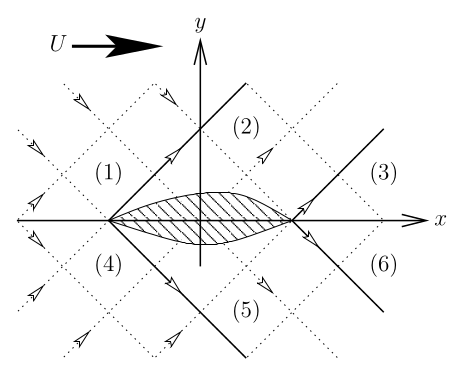
\includegraphics[width=0.25\textwidth]{supersonic}
\end{wrapfigure}

(Causality) Upstream undisturbed: $\phi \stackrel{x \rightarrow -\infty}{\rightarrow} 0$ (Char: $F(x-By) = \const$, $G(x+By) = \const$ on $x\mp By = \const$ resp)
$\Longrightarrow F = C$,
$G=-C$ (where $C=\const$)
on char from $x=-\infty$
$\Longrightarrow \phi \equiv 0$ (1),(4)


On (2), char $x+By=\const$ from $x=-\infty$
$\Longrightarrow G=-C$, and
cond on $y=0_+$
$\Longrightarrow -BF'(x) = Uf_+ '(x)$

$\Longrightarrow \phi_+ (x,y) = -\frac{U}{B}\left( f_+ (x-By) - f_+(-a) \right)$ (2) with continuity with (1)

Similar: $\phi_-(x,y) = \frac{U}{B}\left( f_-\left( x+By \right) - f_-(-a) \right)$ (5)

$\phi = C_1 = -U\left( f_+ (a) - f_+ (-a) \right)/B$ in (3) by continuity with (2)

$\phi = C_2 = U\left( f_- (a) - f_{-}\left( -a \right) \right)$ in (6) by continuity with (5)

\Parsep

\textbf{Nonlinear Waves}
(i) $\frac{D\rho}{Dt} = -\rho u_x$
(ii) $\frac{Du}{Dt} = -\frac{1}{\rho}p_x$
(iii) $\rho c_v \frac{DT}{Dt} = -p u_x$
(iv) $p = \rho RT$
(v) $\gamma = 1 +\frac{R}{c_v}$

\underline{1D Gas Dynamics} 
If $\rho_0$, $p_0$ (init, uniform), then $\frac{p}{\rho^\gamma} = \frac{p_0}{\rho_0^{\gamma}}$
Pf) $\frac{D}{Dt}(\frac{p}{\rho^{\gamma}}) = 
\frac{1}{\rho^{2\gamma}} \left( \frac{Dp}{Dt} \rho^{\gamma} - p\gamma \rho^{\gamma - 1} \frac{D\rho}{Dt} \right) = 
\frac{1}{\rho^\gamma} \left( \frac{Dp}{Dt} - \frac{p \gamma}{\rho}\frac{D\rho}{Dt} \right) \stackrel{\text{(iv)}}{\Longrightarrow}
\rho^\gamma \frac{D}{Dt}\left( \frac{p}{\rho^\gamma} \right) = R\rho \frac{DT}{Dt} + RT \frac{D\rho}{Dt} - \gamma R T \frac{D\rho}{Dt} \stackrel{\text{(1),(3)}}{=}
-\frac{R p u_x}{c_v} + (\gamma - 1)\rho RT u_x \stackrel{\gamma - 1 = \frac{R}{c_v}}{=} 0
$

\underline{Derivation}: \emph{speed of sound} $c^2 \coloneqq \frac{dp}{d\rho} = \frac{\gamma p_0 \rho^{\gamma - 1}}{\rho_0^\gamma} \Rightarrow
\rho = \left( \frac{\rho_0^\gamma}{\gamma p_0} \right)^{1/\left( \gamma - 1 \right)} c^{2/\left( \gamma - 1 \right)}$,
$p = \left( \frac{\rho_0^\gamma}{\gamma p_0} \right)^{1/\left( \gamma - 1 \right)}\frac{c^{2\gamma / \left( \gamma - 1 \right)}}{\gamma}$

$\rho_t + u \rho_x + \rho u_x = 0 \Longrightarrow \frac{2}{\gamma - 1}\left( c_t + u c_x \right) + c u_x = 0$,
$u_t + u u_x + \frac{1}{\rho}p_x = 0 \Longrightarrow u_t + u u_x + \frac{2}{\gamma - 1}c c_x = 0$

Add and subtract to get $\frac{\partial}{\partial t}\left( u \pm \frac{2c}{\gamma - 1}  \right)+ \left( u \pm c \right) \frac{\partial}{\partial x} \left( u \pm \frac{2c}{\gamma - 1} \right) = 0 \Longrightarrow
\frac{d}{dt}\left( u \pm \frac{2c}{\gamma - 1} \right) = 0$ on $\dot x = u \pm c$

\underline{Shallow water theory} Rigid base $z=0$, free surface $z=h(x,t)$ vel field $\uv = u(x,z,t) \mathbf{e}_x + w(x,z,t) \mathbf{e}_z$

Mass Conservation $u_x + w_z = 0$, 
KBC: $w=0$ on $z=0$, $\frac{D}{Dt}(z-h) = 0 \Longrightarrow w = h_t + u h_x$ on $z=h$

Mass Cons $\stackrel{\text{int wrt } z}{\Longrightarrow} h_t + {\left( h \bar u \right)}_{x} = 0$ where $\bar u = \frac{1}{h}\int_0^h u dz$

Assume hydrostatic: $p = p_a + \rho g \left( h-z \right)$, irrotational: $\frac{\partial u}{\partial z} - \frac{\partial w}{\partial x} = 0$

Assume: $|w| \ll |u|$, $\bar u \approx u$, so $h_t+u h_x + h u_x = 0$, $u_t + u u_x + g h_x = 0$. $c = \sqrt{gh}\Longrightarrow\gamma=2$ form.

\Parsep

\textbf{Shock Waves} Frame moving with the shock to fixed frame: $u_\pm \rightarrow u_\pm - V$

\underline{1D Gas Dynamics}
(i) $\left[ pu \right]_-^+ = 0$ \tab
(ii) $\left[ p + \rho u^2 \right]_-^+ = 0$ \tab
(iii) $\left[ \frac{u^2}{2} + \frac{\gamma p}{\left( \gamma - 1 \right)\rho} \right]_-^+ = 0$

Entropy must increase: $M=\frac{u}{c}$, $M_{-}^{2} > 1$ and $M_+^2 < 1$ (Supersonic to subsonic)

\underline{Shallow Water Theory}
(i) $\left[ hu \right]_-^+ = 0$ \tab
(ii) $\left[ hu^2 + \frac{gh^2}{2} \right]_-^+ = 0$

Energy Flow out of jump: $Q = \left[ \underbrace{\int_0^h (\frac{1}{2}\rho u^2 + \rho g z)u dz}_{\text{KE+PE}} + \underbrace{\int_0^h (p-p_{\text{atm}})u dz}_{\text{work by pres.}} \right]_-^+ $

$ = \left[ \frac{\rho h u^3}{2} + \rho g u h^2 \right]_-^+ = \rho h u \left[ \frac{u^2}{2} + gh \right]_-^+ = \left( \rho h u \right)\frac{g\left( h_- - h_+ \right)^3}{4 h_+ h_-} < 0$

\underline{Weak Sol \& RH Cond} $\frac{\partial \mathbf{P}}{\partial t} + \frac{\partial \mathbf{Q}}{\partial x} = \mathbf{0}$,
$\oint_C \mathbf{Q} dt - \mathbf{P} dx$,
$V = \frac{dx}{dt} \Longrightarrow \left[ \mathbf{Q} \right]_-^+ = V \left[ \mathbf{P} \right]_-^+$

Gas Dynamics: $\uv = (\rho, u, p)$, $\mathbf{P} = ({\rho,\rho u, \rho u^2/2 + p/\left( \gamma - 1 \right)})$, $\mathbf{Q} = \left( \rho u, \rho u^2 + p, \rho u^3 / 2 + \gamma p u / \left( \gamma - 1 \right) \right)$

Shallow Water: $\uv = \left( h,u \right)$, $\mathbf{P} = \left( h, hu \right)$, $\mathbf{Q} = \left( uh, hu^2 + gh^2 / 2 \right)$

\end{document}
